\section{Алгоритм создания перечня элементов}

Алгоритм получения перечня элементов по ГОСТ средствами \LaTeX и Python представлен на рисунке~\ref{f:diagram}.

\begin{figure} [H] 
  \centering
  %\documentclass[columnsxxiv,columnsxxvii,pointsubsection]{eskdtext}
%\usepackage{eskdfreesize}	% вставка формата А3
%
%%%% eskdx
\usepackage{eskdchngsheet}		% вставка листа регистрации изменений
\usepackage{eskdfreesize}		% вставка листов нестандартного формата

%%% математика
\usepackage{amsmath,amssymb}
\usepackage{gensymb}			% знак градуса командой \degree
\usepackage{icomma}				% запятая в десятичных дробях

%%% русский язык
\usepackage[T2A]{fontenc}		% кодировка вывода с поддержкой русских букв
\usepackage[utf8]{inputenc}		% кодировка ввода utf8
\DeclareUnicodeCharacter{B1}{$\pm$}
\DeclareUnicodeCharacter{B0}{\degree~C}
\DeclareUnicodeCharacter{B5}{$\mu$}
\usepackage[russian]{babel}		% языки: русский
% выбор русского шрифта TimesNewRoman или Literaturnaya
\IfFileExists{pscyr.sty}{%
	\usepackage{pscyr}\renewcommand{\rmdefault}{ftm}}%
	{\usepackage{literat}}
% решение проблемы копирования текста в буфер обмена
\input glyphtounicode.tex
\input glyphtounicode-cmr.tex	% from pdfx package
\pdfgentounicode=1
\usepackage{cmap}				% улучшенный поиск русских слов в полученном pdf-файле

%%% списки
\usepackage{enumitem}

%%% таблицы
\usepackage{booktabs}			% книжные таблицы
\usepackage{multirow}			% команда для объединения строк
\usepackage{longtable,tabu}		% сложные и длинные таблицы
\usepackage{float}				% опция [H] для точного размещения плавающих объектов
\usepackage{setspace}			% отключает полуторный интервал в окружениях table, figure, предоставляет окружение spacing{} и команды \doublespacing и др.

%%% рисование
\usepackage[europeanresistors,americaninductors]{circuitikz} % рисование электрических схем (автоподключение tikz)
\usetikzlibrary{shapes,arrows.meta,chains} % библиотеки tikz
\usepackage{picture} %
\usepackage{atbegshi} %

%%% базы данных
\usepackage{csvsimple}
%\newcommand{\csvloopx}[2][]{\csvloop{#1,#2}}
%\newcommand{\csvautotabularx}[2][]{\csvloopx[#1]{autotabular={#2}}}
%\newcommand{\respectpercent}{\catcode`\%=12\relax}

%%% листинги
\usepackage{verbatim}
% уменьшенный шрифт в листинге
\makeatletter
\patchcmd{\@verbatim}
  {\verbatim@font}
  {\verbatim@font\scriptsize}
  {}{}
\makeatother

%%% сылки
\usepackage[hyphens]{url}
\usepackage[ 					% гипертекстовое оглавление в PDF
	bookmarks=true, colorlinks=true, unicode=true
]{hyperref}

\usepackage[russian]{cleveref}	% умные ссылки

%%% микротипографика
\usepackage[final]{microtype}[2016/05/14] % улучшает представление букв и слов в строках			% пакеты
%%%% номер
\newcommand{\org}{МДТР}				% организация
\newcommand{\num}{436618.001}		% децимальный номер изделия
\newcommand{\doc}{ПЭ3}				% код документа

%%% основная надпись
\ESKDtitle{Модуль питания и охлаждения}	% наименование изделия
\ESKDdocName{Перечень элементов}	% наименование документа
\ESKDsignature{\org.\num\doc}		% обозначение документа
\ESKDauthor{Максимов}				% автор
\ESKDchecker{Никитина}				% проверил
\ESKDnormContr{}			        % нормоконтролер
\ESKDapprovedBy{Ярославский}	    % утвердил
%\renewcommand{\ESKDcolumnXfIVname}{Согласов.}
\ESKDcolumnXIfIV{\ }					% согласовал
%\ESKDcolumnIVfI{$\text{О}$}		% литера
\ESKDcolumnXXV{МДТР.436618.001}		        % обозначение документа, в котором впервые записан документ

% согласование документации с заказчиком:
%\ESKDcolumnXXV{МДТР.436618.001}
%\ESKDcolumnXXVIII{\small Б/Н от 30.11.2009} % договор
%\ESKDcolumnXXIX{\small 1/57Р6/43 2013}		% договор
%\ESKDcolumnXXX{\small Согласовано: \hfill }				% данные документы
%%%% eskdx
\renewcommand{\ESKDfontShape}{\upshape}

%%% шрифты листа регистрации изменений
\renewcommand{\ESKDfontTabHead}{\scriptsize}
\renewcommand{\ESKDfontTabBody}{\scriptsize}

%%% стиль заголовков
\ESKDsectStyle{section}{\normalfont}
\ESKDsectStyle{subsection}{\normalfont}
\ESKDsectStyle{subsubsection}{\normalfont}
\ESKDsectSkip{section}{8mm}{8mm}
\ESKDsectSkip{subsection}{8mm}{8mm}
\ESKDsectSkip{subsubsection}{15mm}{15mm}

%%% содержание
% содержание без выделений и отступов
\makeatletter
	\renewcommand{\l@section}{\@dottedtocline{1}{0em}{1.25em}} % секции
	\renewcommand{\l@subsection}{\@dottedtocline{2}{0em}{2em}} % подсекции
\makeatother

%%% таблицы
% команды для интервалов до линий в tabluar и др.
\newcommand\T{\rule{0pt}{2.6ex}} % сверху
\newcommand\B{\rule[-1.2ex]{0pt}{0pt}} % снизу
% интервал до линий в tabu не менее:
\tabulinesep=1.5mm 
% счетчик строк
\newcounter{rowcount}
\newcommand\rownumber{\stepcounter{rowcount}\arabic{rowcount}}
% счетчик столбцов
\newcounter{colcount}
\newcommand\colnumber{\stepcounter{colcount}\arabic{colcount}}
% формат номера для второй шапки longtabu или longtable
\DeclareCaptionLabelFormat{continued}{Продолжение таблицы~#2} 

%%% рисунки
% вертикальная отбивка между подписью и содержимым рисунка
\captionsetup[figure]{skip=10pt}
% подпись рисунка по ГОСТ 2.105, 4.3.1
\DeclareCaptionLabelSeparator*{emdash}{~--- }
\captionsetup[figure]{labelsep=emdash}

%%% списки
% стиль списков с абзацным отступом
\setlist{nolistsep, leftmargin=0cm, itemindent=2.2cm} % стиль списков 1 уровня
\setlist[2]{leftmargin=17mm} % стиль списков 2 уровня
% новый стиль списка для пояснений элементов схем
\newlist{picdescription}{enumerate}{1}
\setlist[picdescription]{%
	before={\vspace{10pt}\small},%
	font=\small,%
	label={\arabic* ---},%
	ref={\arabic*},%
	leftmargin=2cm,%
	itemindent=0cm,%
	rightmargin=1cm,%
	labelsep=\widthof{\ },%
	nolistsep}
% нумерация списков:
%% кириллические буквы для 1 уровня
\makeatletter 
	\AddEnumerateCounter{\asbuk}{\@asbuk}{м)}
\makeatother
\renewcommand{\labelenumi}{\asbuk{enumi})}
%% арабские цифры для 2 уровня
\renewcommand{\labelitemii}{\arabic{enumii})}
% используем короткое тире (endash) для ненумерованных списков (ГОСТ 2.105-95, пункт 4.1.7, требует дефиса, но так лучше смотрится)
\renewcommand{\labelitemi}{\normalfont\bfseries{--}}

% размещение float объекта сверху float-only страницы, а не по середине
\makeatletter
	\setlength{\@fptop}{0pt}
	\setlength{\@fpbot}{0pt plus 1fil}
\makeatother

% исправление ситуации с обновленным babel-russian, в котором больше не поддерживается \No (в новых документах следует использовать \textnumero)
\newcommand{\No}{\textnumero}				% настройки стиля
%% -------------------------------------------------
% Set up a new layer for the debugging marks, and make sure it is on
% top
\pgfdeclarelayer{marx}
\pgfsetlayers{main,marx}
% A macro for marking coordinates (specific to the coordinate naming
% scheme used here). Swap the following 2 definitions to deactivate
% marks.
\providecommand{\cmark}[2][]{\relax} 
\providecommand{\cmark}[2][]{%
  \begin{pgfonlayer}{marx}
    \node [nmark] at (c#2#1) {#2};
  \end{pgfonlayer}{marx}
  }
% -------------------------------------------------				% настройки документа
%
%\graphicspath{{images/}}
%
%\begin{document}
%	
%	\newcommand{\dut}{\ESKDtheTitle}		% наименование изделия
\newcommand{\RN}{\org.\num}				% обозначение (децимальный номер) изделия
\newcommand{\hashalg}{CRC-32}			% алгоритм хэш-суммы
\newcommand{\hashsum}{72941475}			% хэш-суммма файла
\newcommand{\file}{\num.cam}			% файл	% сокращения
%% =================================================
% Start the picture
\begin{tikzpicture}[%
    start chain=going below,    % General flow is top-to-bottom
    node distance=6mm and 5cm,	% Global setup of box spacing
    every join/.style={norm},   % Default linetype for connecting boxes
    ]
% ------------------------------------------------- 
% A few box styles 
% <on chain> *and* <on grid> reduce the need for manual relative
% positioning of nodes
\tikzset{
  node font=\small,
  execute at begin node=\setlength{\baselineskip}{1\baselineskip},
  base/.style={draw, on chain, on grid, align=center, minimum height=4ex},
  proc/.style={base, rectangle, text width=8em},
  test/.style={base, diamond, aspect=2, text width=6em},
  term/.style={proc, rounded corners},
  prog/.style={base,rectangle split, rectangle split horizontal,rectangle split parts=3},
  prep/.style={base, chamfered rectangle, chamfered rectangle xsep=2cm},
  manu/.style={base, trapezium, shape border rotate=180, text width=8em},
  % comments
  comm/.style={rectangle, on chain, on grid, text width=8.5cm, xshift=2.5cm},
  % coord node style is used for placing corners of connecting lines
  coord/.style={coordinate, on chain, on grid, node distance=6mm and 2.5cm},
  % nmark node style is used for coordinate debugging marks
  nmark/.style={draw, cyan, circle, font={\sffamily\bfseries}},
  % -------------------------------------------------
  % Connector line styles for different parts of the diagram
  norm/.style={->, draw},
  free/.style={->, draw},
  cong/.style={->, draw},
}
% -------------------------------------------------
% Start by placing the nodes
\node [proc] (p0) {Экспортировать из САПР ПЭ в виде файла \texttt{bom.csv}};
% Use join to connect a node to the previous one 
%\node [proc, join] (p1) {Пересохранить \texttt{bom.csv} в кодировке <<UTF-8 without BOM>>};
\node [prog, join] (p2) {\nodepart[text width=8em]{two} Запустить скрипт \texttt{bomlatex.py}};
%\node [proc, join] (p3) {Заполнить данные ЕСКД в файл \texttt{data.tex}};
\node [term, join] (p4) {Скомпилировать \texttt{bomlatex.tex} компилятором PDFLaTeX 2 раза};
% No join for exits from test nodes - connections have more complex
% requirements
% We continue until all the blocks are positioned
% -------------------------------------------------
% Now we place the coordinate nodes for the connectors with angles, or
% with annotations. We also mark them for debugging.
  
% -------------------------------------------------
% A couple of boxes have annotations
%\node [above=0mm of p4] {(Queue was empty)};
%\node [above=0mm of p8] {(Queue was not empty)};
% -------------------------------------------------
% All the other connections come out of tests and need annotating
% First, the straight north-south connections. In each case, we first
% draw a path with a (consistently positioned) annotation node, then
% we draw the arrow itself.

% ------------------------------------------------- 
% Now the straight east-west connections. To provide consistent
% positioning of the test exit annotations, we have positioned
% coordinates for the vertical part of the connectors. The annotation
% text is positioned on a path to the coordinate, and then the whole
% connector is drawn to its destination box.

% -------------------------------------------------
% Finally, the twisty connectors. Again, we place the annotation
% first, then draw the connector

% -------------------------------------------------
% A last flourish which breaks all the rules
%\draw [->,black, dotted, thick, shorten >=1mm]
%  (p9.south) -- ++(5mm,-3mm)  -- ++(27mm,0) 
%  |- node [black, near end, yshift=0.75em]
%    {(When message + resources available)} (p0);
% -------------------------------------------------
% Now comments
%\node [comm, right=of p1](com1) {};
%\draw ([xshift=2.5mm]com1.north west) -- (com1.north west) -- (com1.south west) -- ([xshift=2.5mm]com1.south west);
%\draw [dashed] (p1) -- (com1);
%% -------------------------------------------------
%\node [comm, right=of p2](com2) {};
%\draw ([xshift=2.5mm]com2.north west) -- (com2.north west) -- (com2.south west) -- ([xshift=2.5mm]com2.south west);
%\draw [dashed] (p2) -- (com2);
%% -------------------------------------------------
%\node [comm, right=of p3](com3) {};
%\draw ([xshift=2.5mm]com3.north west) -- (com3.north west) -- (com3.south west) -- ([xshift=2.5mm]com3.south west);
%\draw [dashed] (p3) -- (com3);
%% -------------------------------------------------
%\node [comm, right=of p4](com4) {};
%\draw ([xshift=2.5mm]com4.north west) -- (com4.north west) -- (com4.south west) -- ([xshift=2.5mm]com4.south west);
%\draw [dashed] (p4) -- (com4);
% -------------------------------------------------
\end{tikzpicture}
% =================================================
%\end{document}
% based on:
% Flowcharting techniques for easy maintenance
% Author: Brent Longborough
  \caption{Алгоритм получения перечня элементов по ГОСТ средствами \LaTeX и Python} 
  \label{f:diagram} 
\end{figure}

\section{Пояснения к алгоритму}

Для того, чтобы получить перечень в формате pdf, необходимо
\begin{enumerate}
	\item экспортировать из САПР csv-файл \texttt{bom.csv}, содержащий следующие обязательные колонки данных (без группировки компонентов "--- одна запись на один компонент):

	\begin{table}[h]
		\centering
		\begin{tabular}{ll}
			\toprule
			Свойство & Пояснение \T \\ \midrule
			\texttt{LogicalDesignator} & Позиционное обозначение \T \\
			\texttt{ManufacturerPartNumber} & Наименование компонента \T \\
			\texttt{Manufacturer} & Изготовитель компонента \T \\
			\texttt{Note} & Примечания \T \\
			\texttt{PhysicalPath} & Иерархия функциональной группы (листа) \T \\
			\texttt{FunctionalGroupTitle} & Наименование функциональной группы (листа) \T \\
			\texttt{FirstApply} & Первое применение \T \\
			\texttt{Author} & Кто разработал \T \\
			\texttt{CheckedBy} & Кто проверил \T \\
			\texttt{NormInspection} & Нормоконтролер \T \\
			\texttt{ApprovedBy} & Кто утвердил \T \\
			\texttt{Organization} & Организация \T \\
			\texttt{DocumentNumberE3} & Обозначение документа схемы \T \\
			\texttt{Title} & Наименование документа схемы \T \\ \bottomrule
		\end{tabular}
	\end{table}
и отсортированный по колонке \texttt{PhysicalPath}. %Файл \texttt{bom.csv} должен быть в кодировке <<UTF-8 without BOM>>.
Пример содержания исходного файла представлен на рисунке~\ref{f:bom}. Функциональные группы (листы) должны иметь уникальные буквенно"=цифровые обозначения (Designator), например, \texttt{A1}, присваиваемые вручную при проектировании схемы. Параметр \texttt{FunctionalGroupTitle} должен быть внесен в свойства листа функциональной группы.
	\item запустить скрипт \texttt{bomlatex.py}, который преобразует исходную базу данных в перечень \texttt{bom-gost.csv}, сортированный приближенно к требованиям ГОСТ 2.702-2011, с четырьмя колонками: \texttt{Designator}, \texttt{Name}, \texttt{Quantity}, \texttt{Comment}. То, каким образом будут сгруппированы компоненты, зависит от содержимого таблицы \texttt{cgroups.csv}. Скрипт также создает таблицу \texttt{latex/bom-gost-latex.csv}, адаптированную для последующей обработки в \LaTeX. Пример содержания адаптированного перечня представлен на рисунке~\ref{f:bom-gost-latex}. Данные основной надписи автоматизированно передаются в файл \texttt{/latex/data.tex}. Пример заполнения файла представлен на рисунке~\ref{f:data}.
	\item открыть файл \texttt{bomlatex.tex} в редакторе Texmaker и запустить компиляцию PDFLaTeX два раза (первый раз компилирует файл, второй "--- выводит количество листов). В результате успешной компиляции в директории появится перечень элементов \texttt{bomlatex.pdf} (см. рисунок~\ref{f:pdf}).

\end{enumerate}


\ESKDlandscapeAIII{%
	\begin{figure}[!t]	
		\verbatiminput{bom.csv} %a https://tex.stackexchange.com/questions/275277/verbatiminput-causes-the-rest-of-the-code-to-be-orange-in-the-editor
		\caption{Пример исходной базы данных texttt{bom.csv}}
		\label{f:bom}
	\end{figure}
	
	\begin{figure}[!h]
		\centering
		\begin{minipage}{.5\textwidth}
			\centering
			\verbatiminput{bom-gost-latex.csv} %a https://tex.stackexchange.com/questions/275277/verbatiminput-causes-the-rest-of-the-code-to-be-orange-in-the-editor
			\captionof{figure}{Пример файла \texttt{latex/bom-gost-latex.csv}}
	  		\label{f:data}
		\end{minipage}
		\begin{minipage}{.5\textwidth}
			\centering
			\verbatiminput{../bomlatex/latex/data.tex} %a https://tex.stackexchange.com/questions/275277/verbatiminput-causes-the-rest-of-the-code-to-be-orange-in-the-editor
			\captionof{figure}{Пример заполнения файла \texttt{latex/data.tex}}
			\label{f:data}
		\end{minipage}
	\end{figure}
	}

\begin{figure}[p]
	\centering
	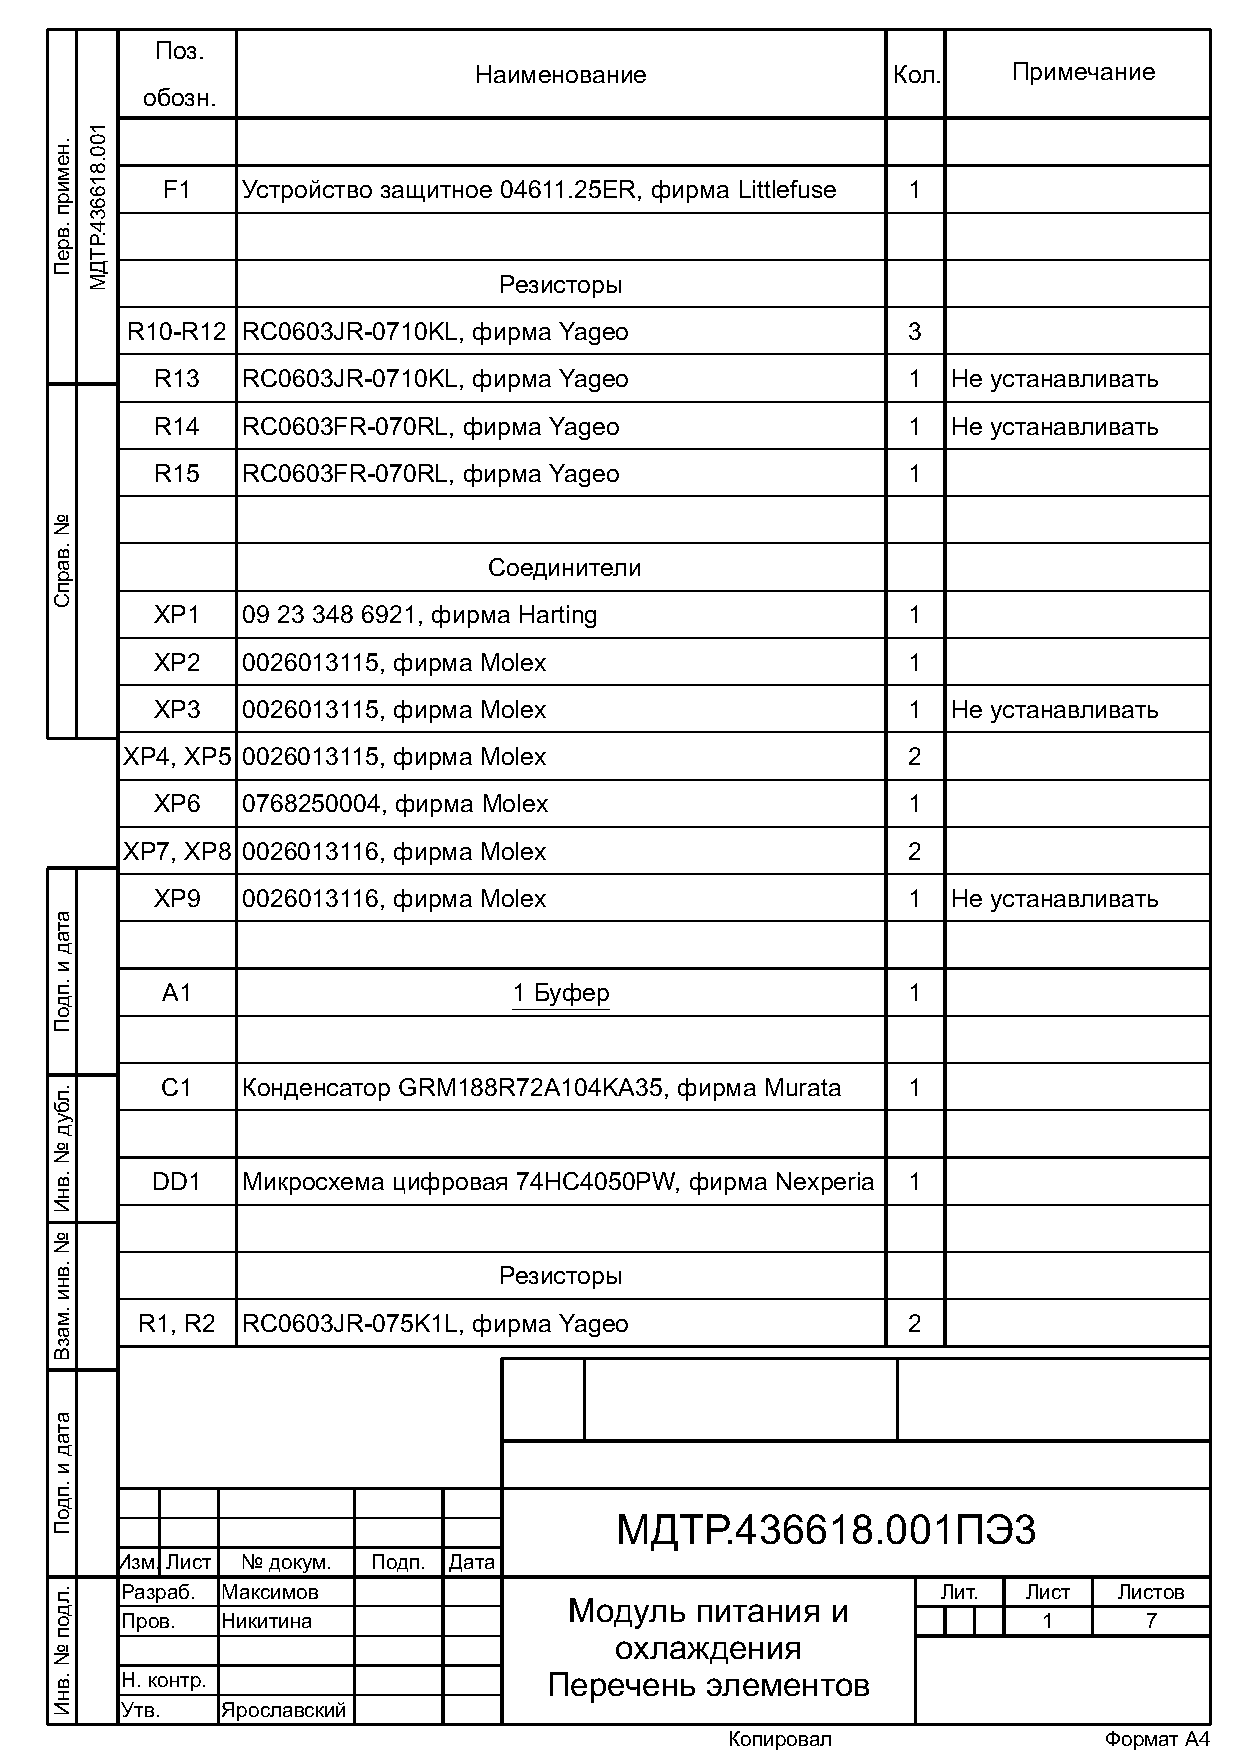
\includegraphics[scale=0.75]{../bomlatex/latex/bomlatex.pdf}
	\caption{Пример перечня элементов, созданного в \LaTeX}
	\label{f:pdf}
\end{figure}
